% Тип документа
\documentclass[a4paper,12pt]{extarticle}

% Шрифты, кодировки, символьные таблицы, переносы
\usepackage{cmap}
\usepackage[T2A]{fontenc}
\usepackage[utf8x]{inputenc}
\usepackage[russian]{babel}

% Это пакет -- хитрый пакет, он нужен но не нужен
\usepackage[mode=buildnew]{standalone}

\usepackage
	{
		% Дополнения Американского математического общества (AMS)
		amssymb,
		amsfonts,
		amsmath,
		amsthm,
		physics,
		% misccorr,
		% 
		% Графики и рисунки
		wrapfig,
		graphicx,
		subcaption,
		float,
		tikz,
		tikz-3dplot,
		caption,
		csvsimple,
		color,
		booktabs,
		pgfplots,
		pgfplotstable,
		geometry,
		% 
		% Таблицы, списки
		makecell,
		multirow,
		indentfirst,
		%
		% Интегралы и прочие обозначения
		ulem,
		esint,
		esdiff,
		% 
		% Колонтитулы
		fancyhdr,
	}  

\usepackage{xcolor}
\usepackage{hyperref}

 % Цвета для гиперссылок
\definecolor{linkcolor}{HTML}{000000} % цвет ссылок
\definecolor{urlcolor}{HTML}{799B03} % цвет гиперссылок
 
\hypersetup{pdfstartview=FitH,  linkcolor=linkcolor,urlcolor=urlcolor, colorlinks=true}
% Обводка текста в TikZ
\usepackage[outline]{contour}

% Увеличенный межстрочный интервал, французские пробелы
\linespread{1.3} 
\frenchspacing 

 
\usetikzlibrary
	{
		decorations.pathreplacing,
		decorations.pathmorphing,
		patterns,
		calc,
		scopes,
		arrows,
		fadings,
		through,
		shapes.misc,
		arrows.meta,
		3d,
		quotes,
		angles,
		babel
	}


\tikzset{
	force/.style=	{
		>=latex,
		draw=blue,
		fill=blue,
				 	}, 
	%				 	
	axis/.style=	{
		densely dashed,
		blue,
		line width=1pt,
		font=\small,
					},
	%
	th/.style=	{
		line width=1pt},
	%
	acceleration/.style={
		>=open triangle 60,
		draw=magenta,
		fill=magenta,
					},
	%
	inforce/.style=	{
		force,
		double equal sign distance=2pt,
					},
	%
	interface/.style={
		pattern = north east lines, 
		draw    = none, 
		pattern color=gray!60,
					},
	cross/.style=	{
		cross out, 
		draw=black, 
		minimum size=2*(#1-\pgflinewidth), 
		inner sep=0pt, outer sep=0pt,
					},
	%
	cargo/.style=	{
		rectangle, 
		fill=black!70, 
		inner sep=2.5mm,
					},
	%
	caption/.style= {
		midway,
		fill=white!20, 
		opacity=0.9
					},
	%
	}

\newenvironment{tikzpict}
    {
	    \begin{figure}[htbp]
		\centering
		\begin{tikzpicture}
    }
    { 
		\end{tikzpicture}
		% \caption{caption}
		% \label{fig:label}
		\end{figure}
    }


\newcommand{\vbLabel}[3]{\draw ($(#1,#2)+(0,5pt)$) -- ($(#1,#2)-(0,5pt)$) node[below]{#3}}
\newcommand{\vaLabel}[3]{\draw ($(#1,#2)+(0,5pt)$) node[above]{#3} -- ($(#1,#2)-(0,5pt)$) }

\newcommand{\hrLabel}[3]{\draw ($(#1,#2)+(5pt,0)$) -- ($(#1,#2)-(5pt,0)$) node[right, xshift=1em]{#3}}
\newcommand{\hlLabel}[3]{\draw ($(#1,#2)+(5pt,0)$) node[left, xshift=-1em]{#3} -- ($(#1,#2)-(5pt,0)$) }



\newcommand\zi{^{\,*}_i}
\newcommand\sumn{\sum_{i=1}^{N}}

\tikzset{
	coordsys/.style={scale=1.8,x={(1.1cm,-0cm)},y={(0.5cm,1cm)}, z={(0cm,0.8cm)}},
	coordsys/.style={scale=1.5,x={(0cm,0cm)},y={(1cm,0cm)}, z={(0cm,1cm)}}, 
	coordsys/.style={scale=1.5,x={(1cm,0cm)},y={(0cm,1cm)}, z={(0cm,0cm)}}, 
}

\usepgfplotslibrary{units}


% Draw line annotation
% Input:
%   #1 Line offset (optional)
%   #2 Line angle
%   #3 Line length
%   #5 Line label
% Example:
%   \lineann[1]{30}{2}{$L_1$}

\newcommand{\lineann}[4][0.5]{%
    \begin{scope}[rotate=#2, blue,inner sep=2pt, ]
        \draw[dashed, blue!40] (0,0) -- +(0,#1)
            node [coordinate, near end] (a) {};
        \draw[dashed, blue!40] (#3,0) -- +(0,#1)
            node [coordinate, near end] (b) {};
        \draw[|<->|] (a) -- node[fill=white, scale=0.8] {#4} (b);
    \end{scope}
}

\newcommand{\lineannn}[4][0.5]{%
    \begin{scope}[rotate=#2, blue,inner sep=2pt, ]
        \draw[dashed, blue!40] (0,0) -- +(0,#1)
            node [coordinate, near end] (a) {};
        \draw[dashed, blue!40] (#3,0) -- +(0,#1)
            node [coordinate, near end] (b) {};
        % \draw[color=white, color=blue] (a) -- node[fill=white, scale=0.8] {#4} (b);
        \draw[->|] (a)++(-0.3,0) -- (a);
        \draw[->|] (b)++(0.3,0) coordinate (xx) -- (b);
        \draw (xx) node[fill=white, scale=0.8, right] {#4};
    \end{scope}
}

% Круговая стрелка относительно центра (дуга из центра)
\tikzset{
  pics/carc/.style args={#1:#2:#3}{
    code={
      \draw[pic actions] (#1:#3) arc(#1:#2:#3);
    }
  },
  dash/.style={
  	dash pattern=on 5mm off 5mm
  }
}

% Среднее <#1>
\newcommand{\mean}[1]{\langle#1\rangle}

\pgfplotsset{
    % most recent feature set of pgfplots
    compat=newest,
}

% const прямым шрифтом
\newcommand\ct[1]{\text{\rmfamily\upshape #1}}
\newcommand*{\const}{\ct{const}}


\usepackage[europeanresistors,americaninductors]{circuitikz}

% Style to select only points from #1 to #2 (inclusive)
\pgfplotsset{select/.style 2 args={
    x filter/.code={
        \ifnum\coordindex<#1\def\pgfmathresult{}\fi
        \ifnum\coordindex>#2\def\pgfmathresult{}\fi
    }
}}


\usepackage{array}
\usepackage{pstool}


%%%%%%%%%%%%%%%%%%%%%%%%%%%%%%%%%%%%%%%%%%%%%%%%%
\makeatletter
\newif\if@gather@prefix 
\preto\place@tag@gather{% 
  \if@gather@prefix\iftagsleft@ 
    \kern-\gdisplaywidth@ 
    \rlap{\gather@prefix}% 
    \kern\gdisplaywidth@ 
  \fi\fi 
} 
\appto\place@tag@gather{% 
  \if@gather@prefix\iftagsleft@\else 
    \kern-\displaywidth 
    \rlap{\gather@prefix}% 
    \kern\displaywidth 
  \fi\fi 
  \global\@gather@prefixfalse 
} 
\preto\place@tag{% 
  \if@gather@prefix\iftagsleft@ 
    \kern-\gdisplaywidth@ 
    \rlap{\gather@prefix}% 
    \kern\displaywidth@ 
  \fi\fi 
} 
\appto\place@tag{% 
  \if@gather@prefix\iftagsleft@\else 
    \kern-\displaywidth 
    \rlap{\gather@prefix}% 
    \kern\displaywidth 
  \fi\fi 
  \global\@gather@prefixfalse 
} 
\newcommand*{\beforetext}[1]{% 
  \ifmeasuring@\else
  \gdef\gather@prefix{#1}% 
  \global\@gather@prefixtrue 
  \fi
} 
\makeatother
%%%%%%%%%%%%%%%%%%%%%%%%%%%%%%%%%%%%%%%%%%%%%%%%%

\geometry		
	{
		left			=	2cm,
		right 			=	2cm,
		top 			=	3cm,
		bottom 			=	3cm,
		bindingoffset	=	0cm
	}

%%%%%%%%%%%%%%%%%%%%%%%%%%%%%%%%%%%%%%%%%%%%%%%%%%%%%%%%%%%%%%%%%%%%%%%%%%%%%%%



	%применим колонтитул к стилю страницы
\pagestyle{fancy} 
	%очистим "шапку" страницы
\fancyhead{} 
	%слева сверху на четных и справа на нечетных
\fancyhead[R]{\labauthors} 
	%справа сверху на четных и слева на нечетных
\fancyhead[L]{Отчёт по лабораторной работе №\labnumber} 
	%очистим "подвал" страницы
\fancyfoot{} 
	% номер страницы в нижнем колинтуле в центре
\fancyfoot[C]{\thepage} 

%%%%%%%%%%%%%%%%%%%%%%%%%%%%%%%%%%%%%%%%%%%%%%%%%%%%%%%%%%%%%%%%%%%%%%%%%%%%%%%

\renewcommand{\contentsname}{Оглавление}

\usepackage{tocloft}
% \renewcommand{\cftpartleader}{\cftdotfill{\cftdotsep}} % for parts
% \renewcommand{\cftsectiondotsep}{\cftdotsep}% Chapters should use dots in ToC
\renewcommand{\cftsecleader}{\cftdotfill{\cftdotsep}}
%\renewcommand{\cftsecleader}{\cftdotfill{\cftdotsep}} % for sections, if you really want! (It is default in report and book class (So you may not need it).
% ---------
% \newcommand{\cftchapaftersnum}{.}%
% \usepackage{titlesec}
% \titlelabel{\thetitle.\quad}
\usepackage{secdot}
\sectiondot{subsection}

\begin{document}

\def\labauthors{Понур К.А., Войтович Д.А}
\def\labgroup{430}
\def\labnumber{1}
\def\labtheme{Многозвенные LC-фильтры}
\renewcommand{\vec}{\mathbf}
\renewcommand{\Re}{\operatorname{Re}}
\renewcommand{\Im}{\operatorname{Im}}
\renewcommand{\phi}{\varphi}
\renewcommand{\hat}{\widehat}

\begin{titlepage}

\begin{center}

{\small\textsc{Нижегородский государственный университет имени Н.\,И. Лобачевского}}
\vskip 1pt \hrule \vskip 3pt
{\small\textsc{Радиофизический факультет}}

\vfill

{\Large Отчет по лабораторной работе №\labnumber\vskip 12pt\bfseries \labtheme}
	
\end{center}

\vfill
	
\begin{flushright}
	{Выполнили студенты \labgroup\ группы\\ \labauthors}%\vskip 12pt Принял:\\ Менсов С.\,Н.}
\end{flushright}
	
\vfill
	
\begin{center}
	Нижний Новгород, \the\year
\end{center}

\end{titlepage}



\tableofcontents
\newpage

\section{Теоретическая часть}
\subsection{Цель работы}

Целью настоящей работы является изучение свойств линейных дискретных систем со многими степенями свободы на примере электрических фильтров. Обычно в качестве фильтров используются цепочки из последовательно соединенных друг с другом идентичных звеньев (четырехполюсников). Такие системы удобно описывать на языке теории волн, интерпретируя их, как направляющие (волноводные) системы. При этом количественное и качественное описание колебательных процессов в фильтрах существенно упрощается и делается более наглядным благодаря использованию таких волновых понятий, как дисперсия, фазовая и групповая скорости волн, коэффициенты отражения плоской волны от границ системы.



\subsection{Уравнения многозвенного электрического фильтра}

Система, состоящая из цепочки идентичных звеньев, будучи системой с пространственной дисперсией, обладает селективными свойствами в определенной области частот. В зависимости от того, какова область частот, в которой колебания пропускаются практически без искажений, фильтры подразделяются на фильтры низких и высоких частот, полосовые и задерживающие фильтры.
\begin{figure}[H]
	\centering
	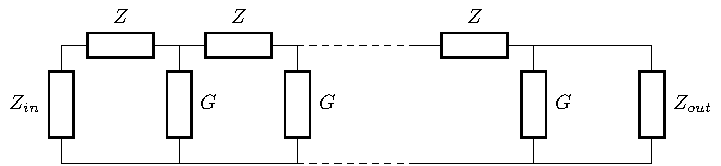
\includegraphics[]{chem/chem1}
	\caption{Общая схема фильтра}
	\label{fig:1}
\end{figure}
Четырехполюсники, образующие звенья рассматриваемых в работе электрических фильтров, состоят из пассивных элементов: индуктивностей, ёмкостей и сопротивлений. Для большей методической простоты мы будем изучать только консервативные фильтры, состоящие из чисто реактивных элементов – индуктивностей и ёмкостей, так называемые LC - фильтры. Общая схема фильтра приведена на рис. \ref{fig:1}, где введены следующие обозначения:  $Z(p)$ – 
$\hyperref[def:1]{\text{операторный импеданс}}$,   $G(p)$– $\hyperref[def:2]{\text{операторная проводимость}}$,   и  $Z_{in}(p)$ и $Z_{out}(p)$ – операторные импедансы на входе и выходе фильтра, соответственно, где $\omega$ – частота колебаний. При расчетах фильтры могут быть разбиты на так называемые Г-образные, Т- образные и П-образные звенья. Заметим, что такое деление -- чисто условное и не влияет на коэффициент передачи рассчитываемого фильтра.
% \begin{figure}[H]
% 	\centering
% 	\includegraphics[]{ris/ris.jpg}
% 	\caption{Общая схема фильтра}
% 	\label{fig:figure1}
% \end{figure}

Рассмотрим для примера фильтр, разбитый на Т-образные звенья (см. рис. \ref{fig:2}), и запишем для него операторные уравнения квазистатики.

\begin{figure}[H]
	\centering
	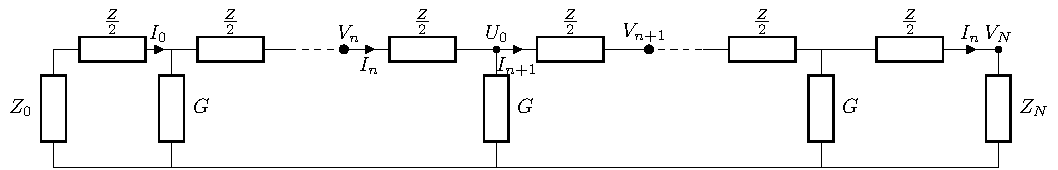
\includegraphics[]{chem/chem2}
	\caption{Фильтр из Т-образных звеньев}
	\label{fig:2}
\end{figure}

При этом на основании законов Кирхгофа для комплексных амплитуд напряжений $V_n$ и токов $I_n$, где $n$ номер звена, будем иметь:
\begin{gather}
\label{eq:2.1}
V_n-U_0=\frac{Z}{2}I_n, \\
U_0-V_{n+1}=\frac{Z}{2}I_{n+1}, \\
GU_0=I_n-I_{n+1}
\end{gather}
Исключая из этих уравнений $U_0$ и разрешая их относительно переменных $V_{n+1}$ и $I_{n+1}$, получим:
\begin{gather}
\label{eq:2.2}
V_{n+1}=a_{11}(p)V_n-a_{12}{p}I_n, \\
I_{n+1}=-a_{21}V_n+a_{22}(p)I_n,
\end{gather}
где
\begin{gather}
\label{eq:2.3}
a_{11}=1+\frac{1}{2}GZ, a_{12}=Z(1+\frac{1}{4}),\\
a_{21}=G, a_{22}=1+\frac{1}{2}GZ
\end{gather}
Отметим следующее важное свойство четырёхполюсников. Четырёхполюсники, для которых выполняются условия
\begin{gather}
\label{eq:2.4}
a_{11}= a_{22},a_{11}^2-a_{12}a_{21}=1,
\end{gather}
называются взаимными.Для них выполняется теорема взаимности, согласно которой свойства четырёхполюсника не изменяются, если его вход и выход поменять ме-стами. Нетрудно видеть, что Т-образное звено представляет собой взаимный четырёхполюсник. В случае П-образного разбиения на звенья в уравнениях (\ref{eq:2.2}) следует положить 
\begin{gather}
a_{11}=1+\frac{1}{2}GZ, a_{12}=Z,\\
a_{21}=G(1+\frac{1}{4}GZ), a_{22}=1+\frac{1}{2}GZ
\end{gather}
Отсюда следует, что П-образное звено также удовлетворяет теореме взаимности. 
Система (\ref{eq:2.2}) должна быть дополнена граничными условиями
\begin{equation}
	\label{eq:2.6}
	V_0=-I_0Z_0, V_N=Z_nI_n
\end{equation}
Исследование явлений, описываемых уравнениями (\ref{eq:2.2}) при условии (\ref{eq:2.6}) включает в себя задачи:
\begin{enumerate}
	\item описание собственных колебаний
	\item описание вынужденных колебаний
\end{enumerate}
Прежде чем переходить к решению первой задачи, исследуем собственные колебания (\ref{eq:2.2}) в безграничной цепочке, положим $N\rightarrow\infty$.

\subsection{Дисперсионное уравнение}
Важнейшей особенностью рассматриваемой цепочной структуры является её периодичность, являющаяся следствием идентичности звеньев и проявляющаяся при $N\rightarrow\infty$ в виде свойства так называемой \textit{трансляционной симметрии}. Это свойство равнозначно свойству инвариантности уравнений (\ref{eq:2.1}) относительно преобразования трансляции $n\Rightarrow n'$ вида $n'=n+m$, где m-- любое целое число. Трансляционная симметрия (\ref{eq:2.1}) в сочетании с линейностью этих уравнений позволяет искать их решение в виде
\begin{equation}
	\label{eq:3.1}
	V_n=Ae^{-in\theta}, I_n=Be^{-in\theta},
\end{equation}
где $n=0,\pm1,\pm2,\dots,$, а $\theta$-- некоторая величина, подлежащая определению. Она находится из условия существования нетривиального решения алгебраической системы
\begin{gather}
\label{eq:3.2}
A(e^{-i\theta}-a_{11})+Ba_{12}=0, \\
Aa_{21}+B(e^{-i\theta}-a_{22})=0,
\end{gather}

получаемой подстановкой (\ref{eq:3.1}) в (\ref{eq:2.2}). Этим условием является равенство нулю детерминанта (\ref{eq:3.2}),что, с учётом (\ref{eq:2.4}), даёт
\begin{equation}
	\label{eq:3.3}
	(e^{-i\theta}-a_{11})^2-a^2_{11}+1=0
\end{equation}
или
\begin{equation}
\label{eq:3.4}
	\cos\theta=a_{11}
\end{equation}

Величина $\theta$, определяемая из (\ref{eq:3.4}) называется \textit{постоянной распространения} и принимает в общем случае комплексные значения ($\theta=\theta'+i\theta''$).
Мнимая часть $\theta$ представляет собой декремент (или инкремент) волны, а действительная часть -- набег фазы волны на одно звено. При этом $\theta'$ связана с длиной волны $\lambda$ очевидным соотношением
\begin{equation}
	\lambda=2 \frac{\pi}{\theta'},
\end{equation}
в котором 
\begin{equation}
	\lambda=min|n_1-n_2|
\end{equation}
где и $n_1$ и $n_2$- номера ячеек, отвечающих синфазным колебаниям. Поскольку параметр является функцией частоты $\omega$, уравнение (\ref{eq:3.4}) связывает постоянную распространения с частотой и называется дисперсионным уравнением системы. Дисперсионное уравнение исчерпывающе характеризует безграничную систему. В случае, когда отсутствует временное и пространственное затухание ($\Im\omega=\Im\theta=0$), оно позволяет определить фазовую ($V_{\text{ф}}$) и групповую ($V_{\text{гр}}$) скорости волн:
\begin{gather}
	V_{\text{ф}}=\frac{\omega}{\theta}, V_{\text{гр}}=\dv{\omega}{\theta}
\end{gather}

\begin{equation*}
	(-\pi \leq\theta\leq\pi)	
\end{equation*}

Дисперсионное уравнение ($\ref{eq:3.4}$) описывает два типа волн -- прямую ($\theta=\theta^+$) и обратную ($\theta=\theta^-$) волну. При этом для фиксированного $\omega$ значения $\theta^+ $и $\theta^-$ будут отличаться только знаком:
\begin{equation}
	\theta^-=-\theta^+.
\end{equation}
Подставляя $\theta^-$ и $\theta^+$ в одно из уравнений системы (\ref{eq:3.2}), можно найти связь между амплитудами напряжения и тока для прямой и обратной волн
\begin{equation}
	\label{eq:3.9}
	B^+=G_xA^+, B^-=-G_xA^-,
\end{equation}
где
\begin{equation}
	G_x=\sqrt{\frac{a_{21}}{a_12}}
\end{equation}
--\textit{характеристическая проводимость фильтра}. Наряду с $G_x$, вводят также и обратную ей величину
\begin{equation}
\label{eq:3.11}
	Z_x=\sqrt{\frac{a_{12}}{a_{21}}},
\end{equation}
именуемую \textit{характеристическим импедансом} фильтра.

Пространственная дисперсия фильтра (описываемая (\ref{eq:3.4})) обуславливает его селективные свойства. Для характеристики этих свойств вводят понятие \textit{полосы прозрачности}, а именно полосы частот, в которой (отсутствует затухание по переменной n).

Найдём связь ширины полосы прозрачности с параметрами фильтра. С этой целью заметим, что поскольку
\begin{equation}
	\sin\theta=\ch\theta''\sin\theta'+i\sh\theta''\cos\theta',
\end{equation}
то в полосе прозрачности
\begin{equation}
	\sin\theta=\sin\theta'.
\end{equation}
Отсюда, в силу (\ref{eq:3.3}), заключаем, что
\begin{equation}
	1-a_{11}^2\geq 0,
\end{equation}
или, с учётом (\ref{eq:2.3}),--
\begin{equation}
	GZ(1+\frac{1}{4}GZ)\leq 0
\end{equation}
Из этого условия и находится полоса прозрачности фильтра. Из него, в частности следует, что в полосе прозрачности фильтра характеристический импеданс (\ref{eq:3.11}) будет действительной величиной.

Вне полосы прозрачности $\sin\theta'=0$ и, следовательно, $\sin\theta=i\sh\theta''$. С учётом (\ref{eq:3.4}), будем иметь
\begin{equation}
	\sh\theta''=\pm\sqrt{a_{11}^2-1}
\end{equation}

\subsection{Собственные колебания}
Найдём собственные колебания в цепочке, состоящей из N одинаковых Т-образных звеньев, описываемой системой уравнений (\ref{eq:2.2}) при граничных условиях (\ref{eq:2.6}). Общее решение такой системы будет представлять собой суперпозицию прямой и обратной волн вида
\begin{gather}
	V_n=A_1e^{-i\theta}+A_2e^{i\theta}, \\
	I_n=B_1e^{-i\theta}+B_2e^{i\theta}.
\end{gather}

Для внутренних звеньев прямая и обратная волны распространяются независимо и для них, в силу (\ref{eq:3.9}), общее решение запишется в виде
\begin{gather}
V_n=A_1e^{-i\theta}+A_2e^{i\theta}, \\
I_n=G_x(A_1e^{-i\theta}+A_2e^{i\theta}).
\end{gather}

Подставляя это решение в граничные условия (\ref{eq:2.6}),
получим следующую однородную систему уравнений для нахождения амплитуд $A_1$ и $A_2$:
\begin{gather}
	(1+Z_0G_x)A_1+(1-Z_0G_x)A_2=0,
	(1-Z_NG_x)e^{-iN\theta}A_1+(1+Z_NG_x)e^{iN\theta}A_2=0.
\end{gather}

Отсюда, расписав условие существования ненулевых решений для $A_1$ и $A_2$, найдём \textit{характеристическое уравнение} рассматриваемой системы
\begin{equation}
\label{eq:4.4}
	1-\Gamma_0\Gamma_Ne^{-2iN\theta}=0,
\end{equation}
где
\begin{equation}
	\Gamma_0\frac{A_1}{A_2}=-\frac{1-Z_0G_x}{1+Z_0G_x}
\end{equation}
--коэффициент отражения от левой границы фильтра, а
\begin{equation}
	\Gamma_N\frac{A_2e^{iN\theta}}{A_1e^{-iN\theta}}=
	-\frac{1-Z_NG_x}{1+Z_NG_x}
\end{equation}
--коэффициент отражения от правой границы фильтра.

Решая совместно дисперсионное уравнение (\ref{eq:3.4}) и характеристическое уравнение (\ref{eq:4.4}), найдём спектр собственных (нормальных) частот фильтра и соответствующий ему спектр значений постоянной распространения $\theta$. Очевидно, что этот спектр будет зависеть не только от параметров звена фильтра, но и от условий на его концах. Отметим также, что число нормальных частот всегда совпадает с числом степеней свободы системы.


\subsection{Вынужденные колебания}
Рассмотрим вынужденные колебания в фильтре, составленном из Т-образных звеньев, при условии, что на входе фильтра действует источник синусоидальной ЭДС $E=E_0\cos(\omega t)$ с внутренним сопротивлением $r_0$ (см. \ref{}). Решение в такой системе можно искать в виде синусоидальных колебаний на частоте внешней силы $\omega$. При этом остаются справедливыми уравнения \eqref{}, а граничные условия принимают вид:
\begin{equation}
	\label{eq:4.1}
	V_0=E_0-r_0Z_0,\;V_N=Z_NI_N.
\end{equation}
\begin{figure}[h!]
	\centering
	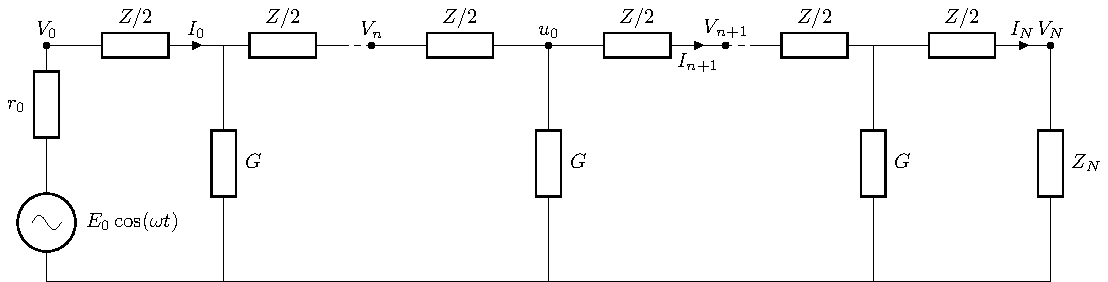
\includegraphics[]{chem/picture3}
	\caption{}
	\label{fig:3}
\end{figure}
Подставляя \eqref{eq:3.2} в \eqref{eq:4.1}, получим 
\begin{equation}
	\label{eq:4.2}
	\begin{gathered}
	(1+r_0G_x)A_1+(1-r_0G_x)A_2=E_0\\
	(1-Z_NG_x)e^{-iN\theta}A_1+(1+Z_NG_x)e^{iN\theta}A_2=0
	\end{gathered}
\end{equation}
Отсюда для $A_1$ и $A_2$ будем иметь
\begin{equation}
	\label{eq:4.3}
	\begin{gathered}
	A_1=\frac{1-\Gamma_0}{2}\cdot\frac{E_0}{1-\Gamma_0\Gamma_Ne^{-2iN\theta}},\\
	A_2=\frac{1-\Gamma_0}{2}\cdot\frac{E_0\Gamma_Ne^{-2iN\theta}}{1-\Gamma_0\Gamma_Ne^{-2iN\theta}},\\
	\end{gathered}
\end{equation}
Подставляя \eqref{eq:4.3} в \eqref{eq:3.2}, получим следующие выражения для комплексных амплитуд напряжения $V_n$ и $I_n$ тока в n-ой ячейке:
\begin{equation}
	\label{eq:4.4}
	\begin{gathered}
	V_n=\frac{1-\Gamma_0}{2}\cdot\frac{E_0e^{-in\theta}}{1-\Gamma_0\Gamma_Ne^{-2iN\theta}}\left[1+\Gamma_Ne^{-2i(N-n)\theta}\right],\\
	I_n=\frac{1-\Gamma_0}{2}\cdot\frac{E_0e^{-in\theta}}{1-\Gamma_0\Gamma_Ne^{-2iN\theta}}G_x\left[1-\Gamma_Ne^{-2i(N-n)\theta}\right],\\
	\end{gathered}
\end{equation}
Из \eqref{eq:4.4} следует, что если частота внешней ЭДС совпадает с одной из собственных частот фильтра, то амплитуды напряжений и токов во всех звеньях фильтра принимают бесконечно большие значения (явление резонанса). Очевидно, что это возможно лишь в отсутствии затухания, т. е. при условии $\Im\omega_m=0$. В реальных системах всегда существуют потери ($\omega_m=\omega'_m+i\omega''_m$) и знаменатель в \eqref{eq:4.4} не обращается в ноль. При этом в случае произвольных потерь картина резонанса достаточно сложна и далека от той, какую мы имеем в одиночном резонансном контуре. Однако, при $\omega''_m/\omega'_m<<1$ эта картина существенно упрощается, и влияние потерь можно описать на привычном языке добротности, вводя её для каждой моды отношением
\begin{equation}
\label{eq:4.5}
Q_m=\omega'_m/\omega''_m
\end{equation}
Таким образом, для системы со многими степенями свободы не имеет смысла говорить о добротности системы вообще, необходимо оговаривать, о добротности какой моды идёт речь.

При изучении вынужденных колебаний важную роль играют два семейства статических характеристик: семейство амплитудно-частотных характеристик (АЧХ) и семейство фазо-частотных характеристик (ФЧХ). Эти семейства находятся из выражения для коэффициента передачи, представляющего собой отношение комплексной амплитуды напряжения на выходе фильтра к амплитуде ЭДС на входе, т.е.
\begin{equation}
\label{eq:4.6}
W(\omega)=\frac{V_N(\omega)}{E_0(\omega)}=\frac{(1-\Gamma_0)(1+\Gamma_N)e^{-iN\theta}}{2\left(1-\Gamma_0\Gamma_Ne^{-2iN\theta}\right)}
\end{equation}
По определению АЧХ -- это функция 
\begin{equation}
\label{eq:4.7}
A(\omega)=|W(\omega)|
\end{equation}
а ФЧХ -- функция
\begin{equation}
\label{eq:4.8}
\Phi(\omega)=-argW(\omega)
\end{equation}
Очевидно, что вид того и другого семейства характеристик зависит от условий на концах фильтра.

Рассмотрим влияние этих условий на $A(\omega)$ и $W(\omega)$ в полосе прозрачности фильтра, полагая для простоты, что нагрузка фильтра чисто активная (т. е. $\Gamma_0$ и $\Gamma_N$ –действительные функции). При этом
\begin{equation}
\label{eq:4.9}
A(\omega)=\frac{1-\Gamma_0}{2}\cdot\frac{1+\Gamma_N}
{\sqrt{1-\Gamma_0\Gamma_N\cos2N\theta+\Gamma^2_0\Gamma^2_N}}
\end{equation}
Из полученного выражения следует, что если фильтр согласован на обоих концах ($\Gamma_0=\Gamma_N=0$), то $A(\omega)=1/2$, т.е. напряжение источника ЭДС делится поровну между фильтром и внутренним сопротивлением источника. Если фильтр согласован только на входе ($\Gamma_0=0$), или только на выходе($\Gamma_N=0$), то $A(\omega)=(1+\Gamma_N)/2$ и $A(\omega)=(1-\Gamma_0)/2$, соответственно. Во всех трёх случаях АЧХ не зависит от числа звеньев фильтра.
 
Если фильтр согласован хотя бы на одном из своих концов, а нагрузка на другом конце -- чисто активная, то существенно упрощается и $\Phi(\omega)$:
\begin{equation}
\label{eq:4.10}
\Phi(\omega)=N\theta(\omega)
\end{equation}
Т.е. ФЧХ с точностью до множителя N сводится к дисперсионной характеристике фильтра.

Многозвенные фильтры представляют собой разновидность длинных линий и используются в радиотехнических устройствах в качестве \textit{линий задержки}. Время запаздывания сигнала при прохождении его через фильтр легко оценить для случая узкополосного сигнала при условии, что спектр его лежит в полосе прозрачности фильтра и укладывается в диапазон частот, в котором фазо-частотную характеристику фильтра можно считать линейной. Спектральную плотность такого сигнала на выходе фильтра для прямой волны можно записать в виде
\begin{equation}
\label{eq:4.11}
u_N(\eta)=A_1(\xi)e^{i[(\Omega+\eta)t-N\theta(\Omega+\eta)t]}
\end{equation}
Учитывая, что $|\eta|\leq\Delta\omega$, где $\Delta\omega$ -- полуширина спектра, и принимая во внимание условие узкополосности $\Delta\omega<<\Omega$, разложим в этом выражении нелинейную функцию $\theta(\Omega+\eta)$ в ряд по степеням $\eta$, ограничившись двумя первыми членами:
\begin{equation}
\label{eq:4.12}
\theta(\Omega+\eta)\approx\theta(\Omega)+\left.\frac{d\theta}{d\omega}\right|_\Omega \eta
\end{equation}
При этом выражение \eqref{eq:4.11} примет вид
\begin{equation}
\label{eq:4.13}
u_N(\eta)\approx A_1(\xi)e^{i[\Omega t-N\theta\Omega]}e^{i(t-N\frac{d\theta}{d\omega}\eta)}
\end{equation}
Отсюда следует, что время задержки сигнала при прохождении через N-звенный фильтр равно $\tau_N=N\frac{d\omega}{d\theta} \Omega$. Т.е. групповая скорость $(d\omega\ /d\theta)$ имеет смысл времени запаздывания, приходящегося на одно звено.
\subsection{Фильтр низкой частоты (ФНЧ)}
Вид отдельного звена ФНЧ изображен на рис \ref{fig:1.1}. ФНЧ служит для пропускания колебаний низкой частоты от $\omega=0$ до $\omega_{\text{ср}}$ (\textit{частота "среза"}). Для ФНЧ
\begin{equation}
\label{eq:5.1.1}
Z=i\omega L,\;G=i\omega C.
\end{equation}
\begin{figure}[h!]
	\begin{minipage}{0.49\linewidth}
		\centering
		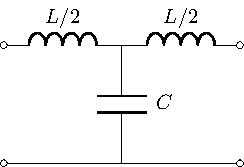
\includegraphics[]{chem/FLF/FLFT.pdf}
		\caption*{Т-образное звено}
	\end{minipage}
\begin{minipage}{0.49\linewidth}
	\centering
	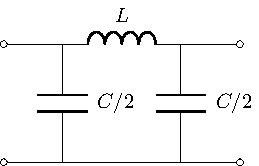
\includegraphics[]{chem/FLF/FLFP.pdf}
	\caption*{П-образное звено}
\end{minipage}
\caption{}
\label{fig:1.1}
\end{figure}
При этом \textbf{диспресионное уравнение} имеет вид 
\begin{equation}
\label{eq:5.1.2}
\omega^2=\frac{2}{LC}(1-\cos\theta)
\end{equation}
\begin{figure}[h!] 
	\centering
	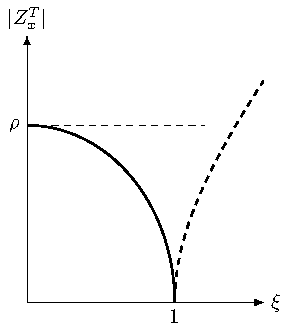
\includegraphics[]{chem/FLF/ZxT.pdf}
	\caption{}
	\label{fig:1.2}
\end{figure}
Из периодического характера этого уравнения следует, что физический смысл имеет лишь та часть дисперсионных ветвей, которая лежит в области $|\theta|\leq\pi$. Т.е. набег фазы на одно звено не может превышать $\pi$. Поскольку постоянная распространения $\theta$ связана с длиной волны $\lambda$ соотношением $\lambda=2\pi/\theta$, то из существования $\theta_{\text{max}}=\pi$ вытекает существо-вание $\lambda_{\text{min}}$. Иными словами, волны с длиной в одну ячейку существовать не могут. Этот результат порождён дискретным характером структуры фильтра и может быть предсказан заранее.

\textbf{Полоса прозрачности} ФНЧ, в силу \eqref{eq:2.15}, задаётся условием
\begin{equation}
\label{eq:5.1.3}
\omega^2\leq\frac{4}{LC}\; (\xi^2=\frac{\omega^2}{\omega^2_{\text{ср}}}\leq1)
\end{equation}

\textbf{Характеристический импеданс} фильтра, состоящего из Т- и П-образных звеньев задаётся соотношениями
\begin{equation}
	Z^T_x=\rho\sqrt{1-\xi^2},\;
	Z^{\text{П}}_x=\frac{\rho}{\sqrt{1-\xi^2}},\;
	(\rho=\sqrt{L/C})
\end{equation}
\begin{figure}[h!]
\begin{minipage}{0.49\linewidth}
	\centering
	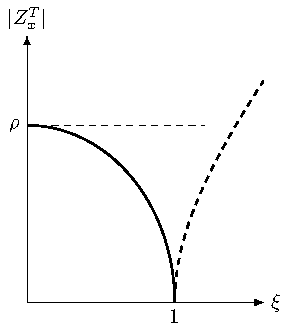
\includegraphics[]{chem/FLF/ZxT.pdf}
\end{minipage}
\begin{minipage}{0.49\linewidth}
	\centering
	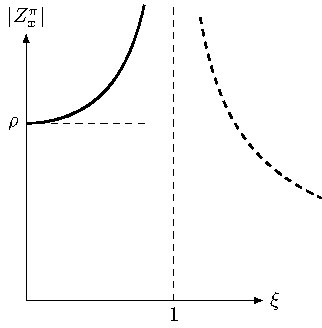
\includegraphics[]{chem/FLF/ZxP.pdf}
\end{minipage}
\caption{}
\label{fig:1.3}
\end{figure}
Соответствующие им частотные зависимости изображены на рис. \ref{fig:1.3}.

\textbf{Параметры звеньев фильтра} рассчитываются по формулам
\begin{equation}
	\label{eq:5.5}
	L=\frac{2\rho}{\omega_{\text{ср}}},\;
	C=\frac{2}{\rho\omega_{\text{ср}}}
\end{equation}
Время задержки на одно звено даётся выражением
\begin{figure}[H]
	\centering
	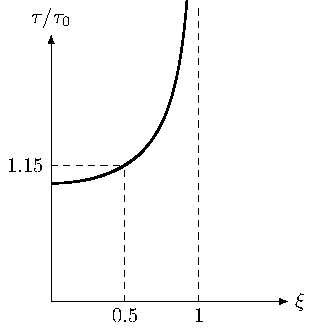
\includegraphics[]{chem/FLF/tau1.pdf}
	\caption{}
	\label{fig:1.4}
\end{figure}
\begin{equation}
\label{eq:5.6}
\tau=\frac{2}{\omega_{\text{ср}}\sqrt{1-\xi^2}}
\end{equation}
Графически зависимость времени задержки от частоты изображена на рис. \ref{fig:1.4}
\section{Фильтр высокой частоты (ФВЧ)} 
Вид отдельного звена ФВЧ изображен на рис \ref{fig:6.1}. ФВЧ служит для пропускания колебаний с частотами $\omega\geq$. Для ФНЧ
\begin{equation}
\label{eq:6.1.1}
Z=i/\omega C,\;G=i/\omega L.
\end{equation}
\begin{figure}[h!]
	\begin{minipage}{0.49\linewidth}
		\centering
		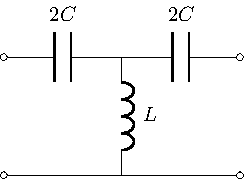
\includegraphics[]{chem/FHF/FHFT.pdf}
		\caption*{Т-образное звено}
	\end{minipage}
	\begin{minipage}{0.49\linewidth}
		\centering
		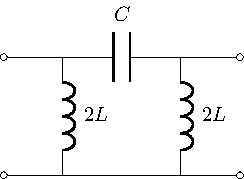
\includegraphics[]{chem/FHF/FHFP.pdf}
		\caption*{П-образное звено}
	\end{minipage}
	\caption{}
	\label{fig:6.1}
\end{figure}
При этом \textbf{диспресионное уравнение} имеет вид 
\begin{equation}
\label{eq:6.1.2}
\omega^2=\frac{1}{2LC(1-\cos\theta)}
\end{equation}
График дисперсионной зависимости приведен на рис. \ref{fig:6.2}
\begin{figure}[h!]
	\centering 
	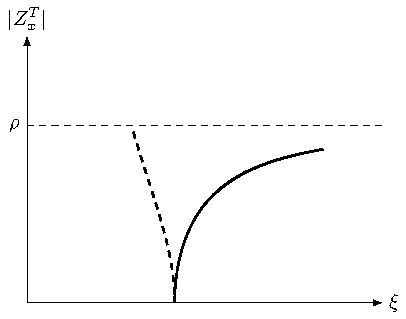
\includegraphics[]{chem/FHF/ZxP2.pdf}
	\caption{}
	\label{fig:6.2}
\end{figure}


\textbf{Полоса прозрачности} ФНЧ, определяется из условия 
\begin{equation}
\label{eq:6.1.3}
1-\frac{1}{4\omega^2LC\geq0}\;(\xi^2\geq1)
\end{equation}

\textbf{Характеристический импеданс} фильтра, состоящего из Т- и П-образных звеньев задаётся соотношениями
\begin{equation}
Z^T_x=\rho\sqrt{1-\frac{1}{\xi^2}},\;
Z^{\text{П}}_x=\frac{\rho\xi}{\sqrt{\xi^2-1}},\;
(\rho=\sqrt{L/C})
\end{equation}
\begin{figure}[h!]
	\begin{minipage}{0.49\linewidth}
		\centering
		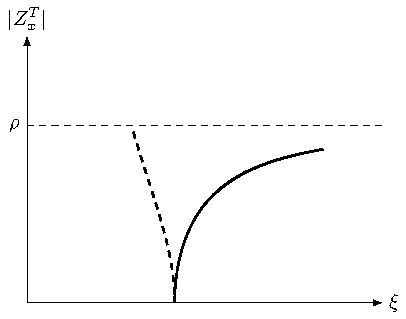
\includegraphics[]{chem/FHF/ZxP2.pdf}
	\end{minipage}
	\begin{minipage}{0.49\linewidth}
		\centering
		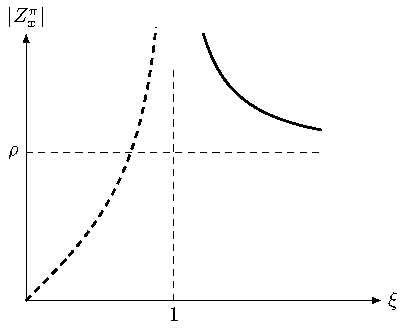
\includegraphics[]{chem/FHF/ZxT2.pdf}
	\end{minipage}
	\caption{}
	\label{fig:6.3}
\end{figure}
Соответствующие им частотные зависимости изображены на рис. \ref{fig:6.3}.

\textbf{Параметры звеньев фильтра} рассчитываются по формулам
\begin{equation}
\label{eq:6.5}
L=\frac{\rho}{2\omega_{\text{ср}}},\;
C=\frac{1}{2\rho\omega_{\text{ср}}}
\end{equation}
Время задержки на одно звено даётся выражением
\begin{figure}[h!]
	\centering
	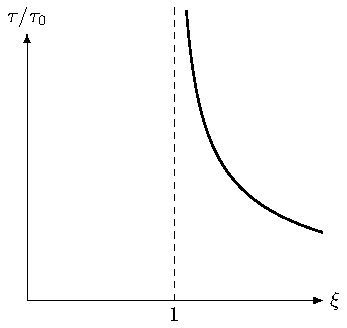
\includegraphics[]{chem/FHF/tau2.pdf}
	\caption{}
	\label{fig:6.4}
\end{figure}
\begin{equation}
\label{eq:6.6}
\tau=\frac{1}{\omega_{\text{ср}}\xi\sqrt{\xi^2-1}}
\end{equation}
Графически зависимость времени задержки от частоты изображена на рис.\ref{fig:6.4}
\subsection{Полосовой фильтр}
Вид отдельного звена полосового фильтра изображен на рис.\ref{fig:7.1}. Полосовой фильтр служит для пропускания колебаний в полосе частот$\omega_1\leq\omega\leq\omega_2$.
\begin{figure}[h!]
	\begin{minipage}{0.49\linewidth}
		\centering
		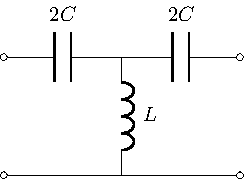
\includegraphics[]{chem/FHF/FHFT.pdf}
		\caption*{Т-образное звено}
	\end{minipage}
	\begin{minipage}{0.49\linewidth}
		\centering
		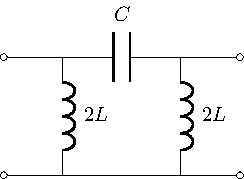
\includegraphics[]{chem/FHF/FHFP.pdf}
		\caption*{П-образное звено}
	\end{minipage}
	\caption{}
	\label{fig:7.1}
\end{figure}
Для полосового фильтра
\begin{equation}
\label{eq:7.1}
Z=i\omega L_1+i/\omega C_1,\;G=i\omega C_2+i/\omega L_2.
\end{equation}
\textbf{Дисперсионное уравнение} полосового фильтра определяется следующей зависимостью
\begin{equation}
	\label{eq:7.2}
	f(\omega^2)=\sin^2\frac{\theta}{2}
\end{equation}
где
\begin{equation}
	\label{eq:7.3}
	f(\omega^2)=\frac{(L_1C_1\omega^2-1)(L_2C_2\omega^2-1)}{4\omega^2L_2C_1}
\end{equation}

\begin{figure}[h!]
	\centering 
	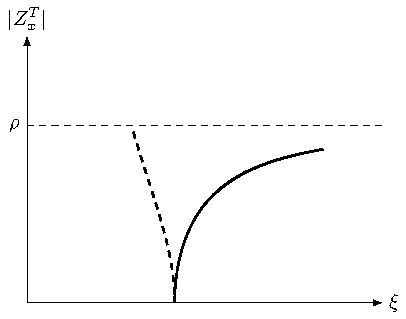
\includegraphics[]{chem/FHF/ZxP2.pdf}
	\caption{}
	\label{fig:7.2}
\end{figure}
Так как $\displaystyle 0\leq\sin^2\frac{\theta}{2}\leq1$, то система будет пропускать частоты $\displaystyle\omega_1\leq\omega\leq\frac{1}{\sqrt{L_1C_1}}$ и $\displaystyle frac{1}{\sqrt{L_1C_1}}\leq\omega\leq\omega_2$. На практике интересен случай, когда $\displaystyle \frac{1}{\sqrt{L_1C_1}}=\frac{1}{\sqrt{L_2C_2}}=\omega_0$, $\displaystyle \frac{L_1}{L_2}=\frac{C_1}{C_2}=\alpha$
При этом дисперсионное уравнение принимает вид
\begin{equation}
\label{eq:7.4}
\left(\frac{\omega^2}{\omega^2_0}-1\right)\frac{\omega_0}{2\omega}\sqrt{\alpha}=\pm\sin\frac{\theta}{2}
\end{equation}
Соответствующие ему дисперсионные кривые изображены на рис.\ref{fig:7.3}
\begin{equation}
\label{eq:7.5}
\omega_1=\frac{\omega_0}{\sqrt{\alpha}}(\sqrt{1+\alpha}-1),\;
\omega_2=\frac{\omega_0}{\sqrt{\alpha}}(\sqrt{1+\alpha}+1)
\end{equation}
%\begin{figure}
%	\includegraphics[]{}
%	\caption{}
%	\label{fig:7.3}
%\end{figure}
\textbf{Полоса прозрачности} фильтра определяется из условия 
\begin{equation}
\label{eq:7.6}
\left(\frac{\omega}{\omega_0}-\frac{\omega_0}{\omega}\right)^2\alpha\leq 4.
\end{equation}
\textbf{Характеристический импеданс фильтра}, состоящего из Т- и П- образных звеньев соотношениями
\begin{equation}
\label{eq:7.7}
Z^T_x=\rho\sqrt{1-\frac{\alpha}{4}\left(\frac{\omega}{\omega_0}-\frac{\omega_0}{\omega}\right)^2},\;
Z^\text{П}_x=\frac{\rho}{\sqrt{1-\frac{\alpha}{4}\left(\frac{\omega}{\omega_0}-\frac{\omega_0}{\omega}\right)^2}}
\end{equation}
где $\rho=\sqrt{L_2/C_1}$. Зависимость этого импеданса от частоты приведена на рис.\ref{fig:7.4}
\begin{figure}
\begin{minipage}{0.49\linewidth}
	\centering
	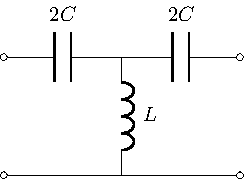
\includegraphics[]{chem/FHF/FHFT.pdf}
\end{minipage}
\begin{minipage}{0.49\linewidth}
	\centering
	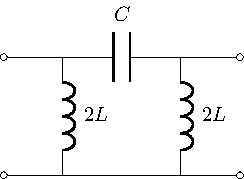
\includegraphics[]{chem/FHF/FHFP.pdf}
\end{minipage}
\caption{}
\label{fig:7.4}
\end{figure}

\textbf{Параметры фильтра} рассчитываются по следующим формулам:
\begin{equation}
\label{eq:7.8}
\begin{gathered}
L_1=\frac{\sqrt{\alpha}\rho}{\omega_0}=\frac{2\rho}{\omega_2-\omega_1},\;
L_2=\frac{L_1}{\alpha}=\frac{\rho(\omega_2-\omega_1)}{2\omega^2_0}\\
C_1=\frac{1}{\omega^2_0L_1}=\frac{\omega_2-\omega_1}{2\rho\omega_1\omega_2},\;
C_2=\alpha C_1=\frac{2}{\rho(\omega_2-\omega_1)}\\
\rho=\sqrt{\frac{L_2}{C_1}}=\sqrt{\frac{L_1}{\alpha C_1}}
\end{gathered}
\end{equation}

\section{Практическая часть}
%%%%%%%%%%%%%%%%%%%%%%%%%%%%%%%%%%%%%%%%%%%%%%%%%%%%%%%%%%%%%%%%%%%%%%%%%%%%%%
\subsection{Фильтр низких частот}
\begin{figure}[H]
	\centering
	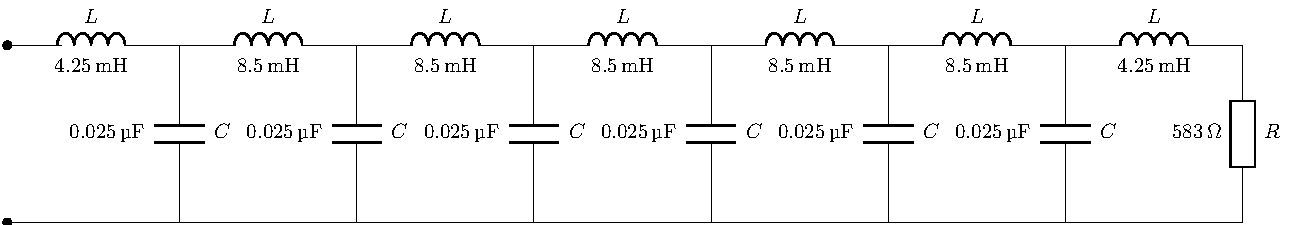
\includegraphics[scale=0.75]{chem/chem3}
	\caption{ Схема использованного ФНЧ из 6-ти Т-образных звеньев}
	\label{fig:chem3}
\end{figure}
Параметры используемого фильтра:
$\nu_{\text{гр}}=21.83 \text{ кГц} ,\,R=583\text{ Ом}$, значения C и L указаны на схеме.

Амплитудно- и фазочастотные характеристики фильтра показаны на рисунках (\ref{fig:figure1}) и (\ref{fig:figure2}) соответственно.
\begin{figure}[h!]
	\centering
	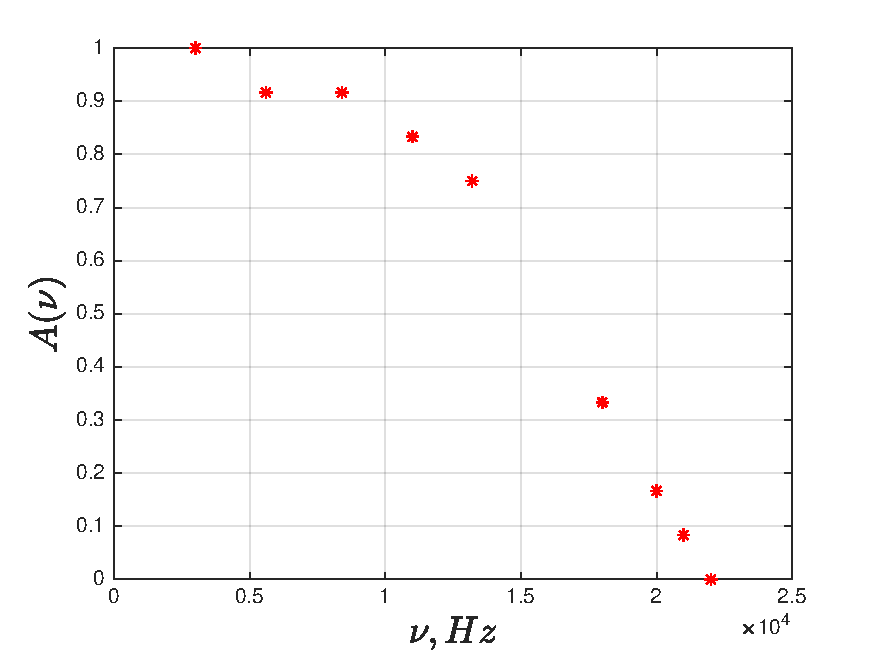
\includegraphics[]{graph/graph1}
	\caption{АЧХ}
	\label{fig:figure1}
\end{figure}

\begin{figure}[h!]
	\centering
	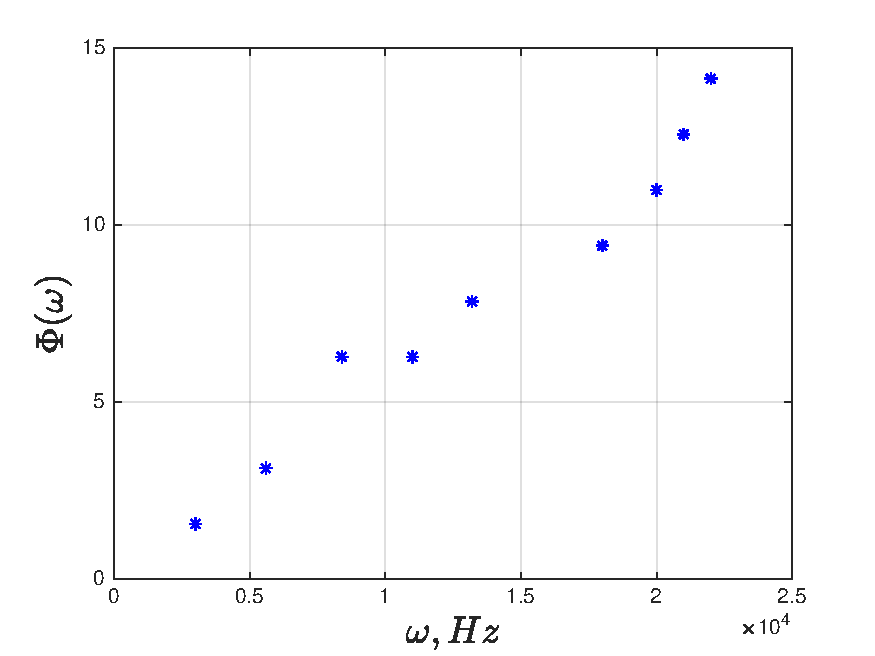
\includegraphics[]{graph/graph2}
	\caption{ФЧХ}
	\label{fig:figure2}
\end{figure}

\begin{table}[H]
\caption{\label{tab:1}Время задержки для сигнала на выходе ФНЧ}
	\begin{center}
		\begin{tabular}{|c|c|}
		\hline
		Число звеньев & Время задержки, мкс \\
		\hline
		6 & 100\\
		5 & 80\\
		4 & 70\\
		3 & 50\\
		2 & 40\\
		1 & 20\\
		\hline
		Среднее (на одно звено) & 60 \\
		\hline
		\end{tabular}
	\end{center}
\end{table}

%%%%%%%%%%%%%%%%%%%%%%%%%%%%%%%%%%%%%%%%%%%%%%%%%%%%%%%%%%%%%%%%%%%%%%%%%%%%%%
\subsection{Фильтр высоких частот}
\begin{figure}[H]
	\centering
	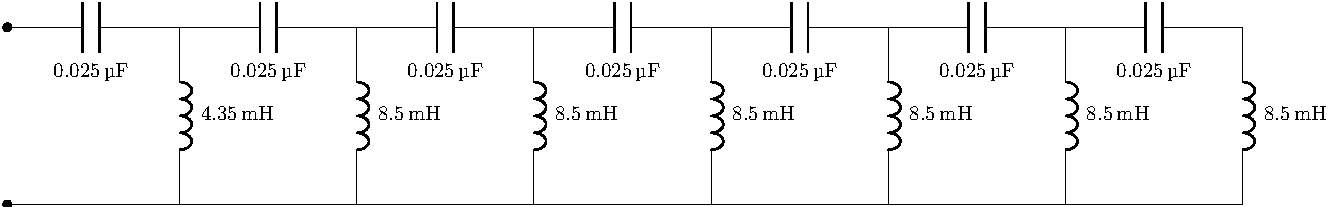
\includegraphics[scale=0.75]{chem/chem5}
	\caption{ Схема использованного ФВЧ из 6-ти Т-образных звеньев}
	\label{fig:4}
\end{figure}
Параметры используемого фильтра: $\nu_{\text{гр}}=7.83$кГц, $R=406$ Ом,$C=0.025$ мкФ,
$L=4.25$ мГн. 

Амплитудно- и фазочастотные характеристики фильтра показаны на рисунках (\ref{fig:figure3}) и (\ref{fig:figure4}) соответственно.
\begin{figure}[h!]
	\centering
	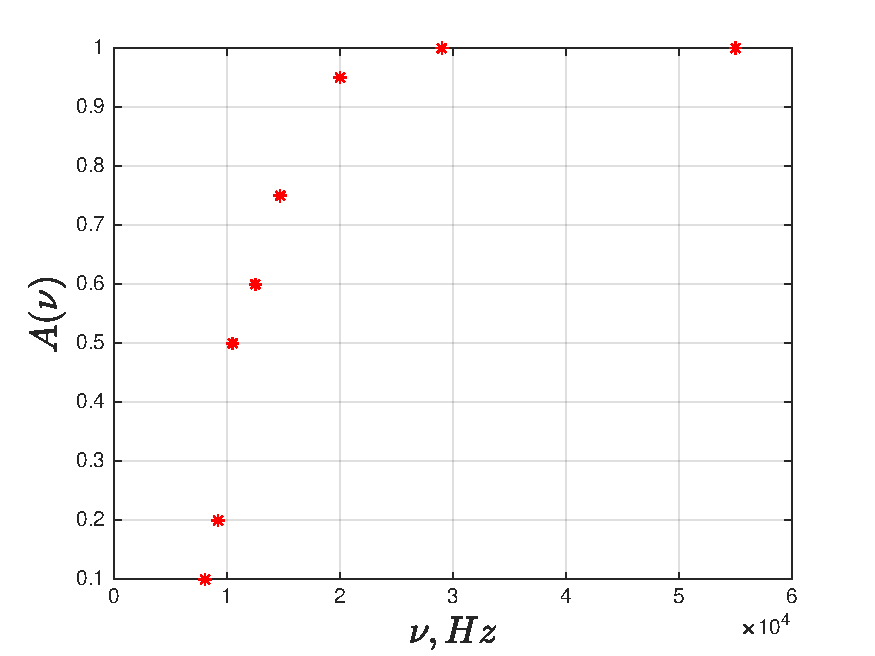
\includegraphics[scale=0.9]{graph/graph3}
	\caption{АЧХ}
	\label{fig:figure3}
\end{figure}

\begin{figure}[h!]
	\centering
	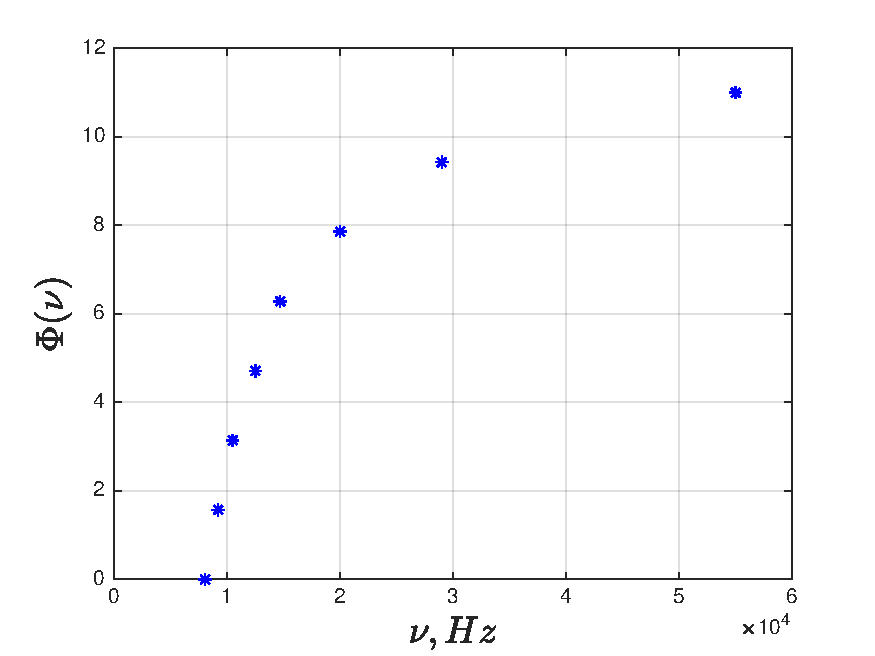
\includegraphics[scale=0.9]{graph/graph4}
	\caption{ФЧХ}
	\label{fig:figure4}
\end{figure}

\begin{figure}[H]
	\centering
	\includegraphics[scale=0.2]{images/1.png}
	\caption{Прохождение прямоугольного импульса через ВЧФ}
	\label{fig:ris1}
\end{figure}

%%%%%%%%%%%%%%%%%%%%%%%%%%%%%%%%%%%%%%%%%%%%%%%%%%%%%%%%%%%%%%%%%%%%%%%%%%%%%%
\subsection{Полосовой фильтр}
\begin{figure}[H]
	\centering
	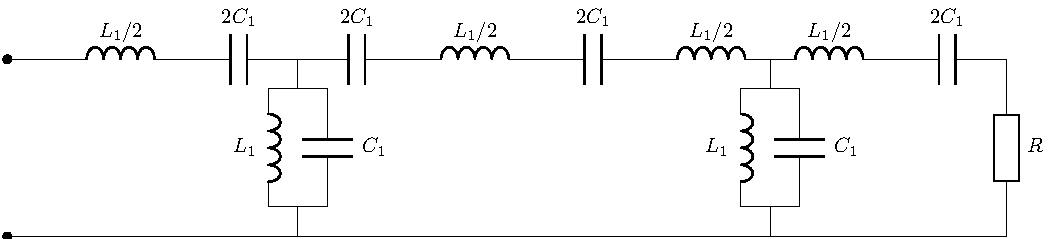
\includegraphics[scale=1]{chem/chem4}
	\caption{ Схема использованного ПФ из 2-х Т-образных звеньев}
	\label{fig:chem4}
\end{figure}
Параметры используемого фильтра: $\nu_1=7.83$ кГц, $\Delta\nu=15.4$ кГц, $R=412$ Ом, $C_1=0.025$ мкФ,
$C_2=0.025$ мкФ, $L_1=8.5$ мГн, $L_2=4.25$ мГн. 

Амплитудно- и фазочастотные характеристики фильтра показаны на рисунках (\ref{fig:figure5}) и (\ref{fig:figure6}) соответственно.

\begin{figure}[H]
	\centering
	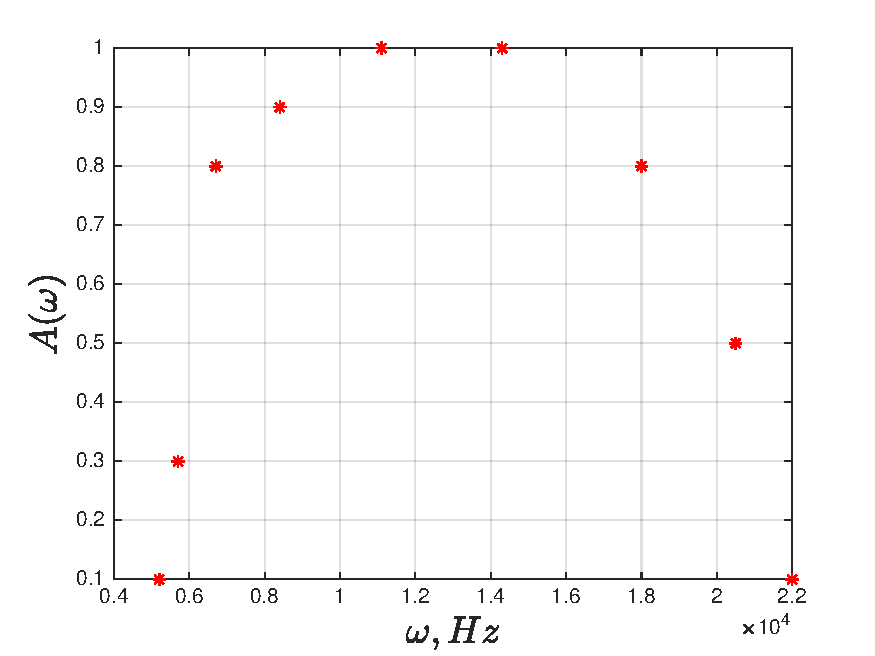
\includegraphics[scale=0.9]{graph/graph5}
	\caption{АЧХ}
	\label{fig:figure5}
\end{figure}

\begin{figure}[H]
	\centering
	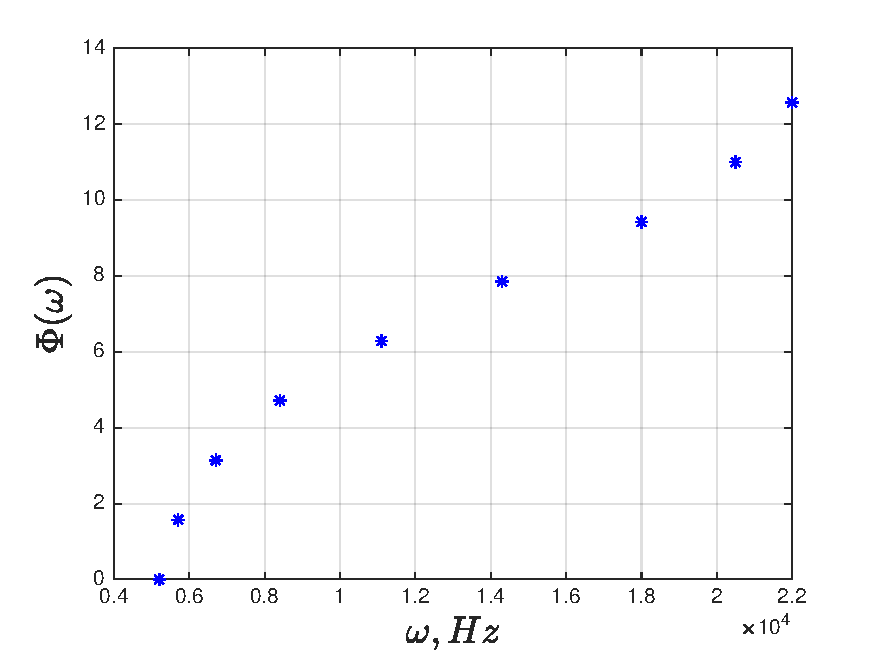
\includegraphics[scale=0.9]{graph/graph6}
	\caption{ФЧХ}
	\label{fig:figure6}
\end{figure}





\begin{figure}[H]
	\centering
	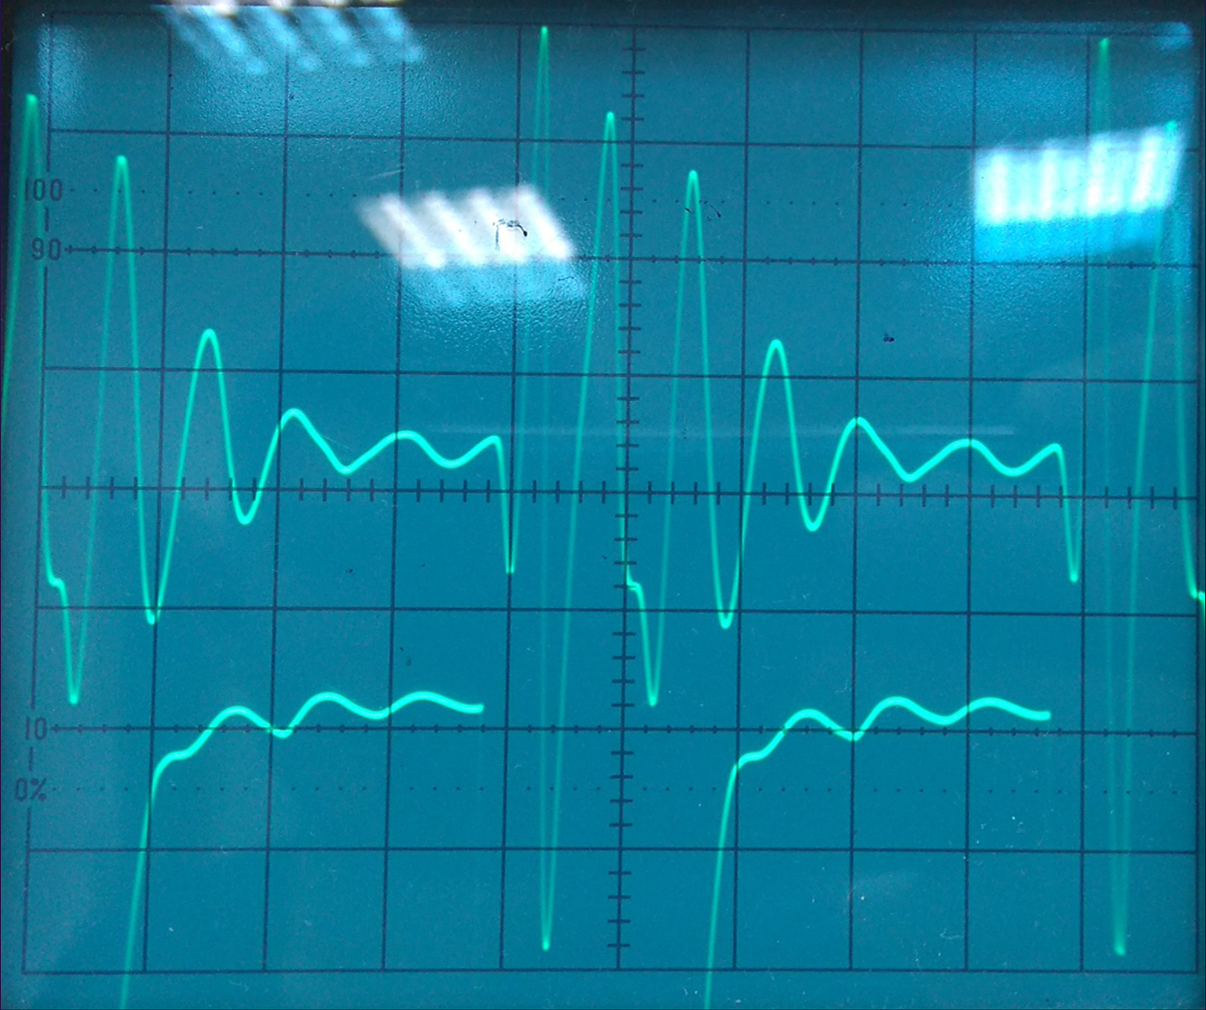
\includegraphics[scale=0.25]{images/2}
	\caption{Прохождение прямоугольного импульса через ПФ}
	\label{fig:ris2}
\end{figure}


% \section{Вопросы}
% \begin{enumerate}
% \item Как снимаются амплитудные и фазовые характеристики фильтров?
% \item Как зависит вид АЧХ и ФЧХ от числа звеньев? Объяснить эту зависимость.
% \item Зачем нужно согласовывать фильтр с нагрузкой? Как практически осуществляется такое согласование?
% \item Какой вид имеют АЧХ и ФЧХ для различных фильтров?
% \item Что такое характеристический импеданс, постоянная распространения, полоса прозрачности фильтра? Чем они определяются?
% \item Что характеризует дисперсионное уравнение? Какой вид имеют дисперсионные характеристики для различных фильтров?
% \item Что такое нормальные частоты? Чем определяется их количество и значения?
% \item Какой вид имеет распределение амплитуд собственных колебаний вдоль фильтра? От чего оно зависит?
% \item Чем отличаются фильтры, собранные из Т-образных звеньев, от фильтров их П-образных звеньев?
% \item При каких условиях сигнал будет проходить через фильтр, задерживаясь, но не искажаясь?
% \item Чем определяется время задержки сигнала на фильтре? Как его измерить?
% \end{enumerate}
% \section{Ответы на вопросы и новые понятия}
% \textit{Операторной функцией} цепи называют отношение изображения реакции к изображению входного воздействия. Обычно, если это не приводит к путанице, слово <<операторный>> опускают. Функции цепи определяют при нулевых начальных условиях, поэтому в операторных схемах замещения индуктивного и емкостного элементов отсутствуют независимые источники.
% Т
% аким образом, операторная функция является изображением реакции цепи
% при нулевых начальных условиях.
% Операторное сопротивление:
% \begin{equation}
% 	\label{def:1}
% 	Z(p)=\frac{U(p)}{I(p)}
% \end{equation}
% Операторная проводимость определяется как обратная величина входного сопротивления:
% \begin{equation}
% \label{def:2}
% 	G(p)=\frac{I(p)}{U(p)}
% \end{equation}


\end{document}